\documentclass{IEEEtran}

\usepackage{mathtools}
\usepackage{graphicx}
\usepackage{subfig}
\usepackage{verbatim}
\usepackage{algpseudocode}
\usepackage{natbib}
\usepackage{url}
\usepackage{listings}
\usepackage[spanish]{babel}
\usepackage[utf8x]{inputenc}
\usepackage{float}

\begin{document}

\title{Simulación y Evaluación de Redes de
Interconexión Nanofotónicas sobre Silicio
para Chips Multiprocesadores}
\date {Abril de 2013}
\author{\IEEEauthorblockN{Tatiana López Guevara, Jose Alfredo Jaramillo\\}
\IEEEauthorblockA{tatiana@sirius.utp.edu.co, jj@sirius.utp.edu.co \\
Universidad Tecnológica de Pereira\\ Grupo de Investigación Sirius \\
 }}
\maketitle


\begin{abstract}
Las redes de interconexión electrónicas, tienen un impacto directo en 
la limitación de potencia, ancho de banda y latencia de los
chips multiprocesadores (CMPs) actuales. 
Estas limitaciones sumadas a la inhabilidad de escalar eficientemente a cientos de
núcleos, la presenta como una solución poco viable a largo plazo.
El empleo de la tecnología de punta que usa la nanofotónica sobre silicio, 
se presenta como una solución prometedora a este
problema, ya que no solo permite el flujo de grandes cantidades de 
datos en una misma línea de transmisión, sino que tiene una facilidad de 
integración con la microelectrónica actual manteniendo al mismo tiempo los 
bajos costes de fabricación, gracias a que se pueden reutilizar las técnicas 
de manufactura de semiconductores tradicionales.
En este proyecto se simularon y evaluaron las redes de interconexión con 
topología C-Mesh nanofotónicas híbridas sobre silicio para chips multiprocesadores 
con el fin de conocer si realmente son más eficiente en términos de consumo de potencia
 y latencia que sus equivalentes electrónicos.
Se utilizó de una metodología estructural, 
en la cual se identificaron 2 grandes etapas: 
Primero se evaló el comportamiento de los elementos básicos que conforman
los dispositivos fotónicos, lo que  permitió tener un
mayor control sobre los parámetros con los que se simula su comportamiento a nivel
de un sistema completo en una capa de abstracción superior, es decir, sobre la siguiente
etapa del proyecto.
La última etapa estuvo encaminada a la simulación del sistema completo para
obtener los análsis comparativos 
en términos de ancho de banda, 
potencia y latencia de la red C-Mesh sobre diferentes conjuntos de pruebas. 
La aplicación de este conocimiento 
científico orientado al área de arquitectura de computadores y a la nanotecnología, 
permitirá la creación de nuevos diseños que aporten a la solución de los
problemas de rendimiento vs potencia, apuntando a mejorar la competitividad 
nacional mediante la generación de producción intelectual en dicho aspecto.
\end{abstract}

\begin{IEEEkeywords}
 Arquitectura de computadores, Silicon Photonics,
Chips Multiprocesadores, Topologías de Interconexión, Simulación.
\end{IEEEkeywords}

\section{Introducción}
\IEEEPARstart{L}{as} tendencias actuales de los procesadores muestran 
que en un periodo corto de tiempo, 
alcanzaremos los cientos de núcleos en un solo chip. 
A medida que la cantidad de estos núcleos aumenta, los requerimientos de ancho de banda 
de las redes de interconexión que permiten la comunicación interna entre estos y 
hacia la memoria, se incrementa. A medida que se incrementa el ancho de banda en 
sistemas de interconexión electrónicos, la latencia y la disipación de poder, 
se ven impactadas considerablemente, por lo que dicha solución se vuelve no viable.

La fusión del campo de la fotónica con la nanotecnología denominado 
nanofotónica, ha permitido el desarrollo de dispositivos
basados en silicio de altas prestaciones y bajo consumo, ya que pueden 
ser producidos usando las técnicas ya existentes de manufacturación de semiconductores, 
y gracias a que el silicio actualmente es utilizado como el componente base 
en la mayoría de circuitos, es posible crear dispositivos híbridos en los cuales 
se integran componentes tanto electrónicos como ópticos en un solo microchip. 
Tomando en cuenta estos últimos avances, las redes de interconexión ópticas 
en un chip o NoCs nano ópticas sobre silicio, ya ha sido conceptualizada, 
permitiendo superar las actuales limitaciones de su equivalente electrónico 
en los chips de multiprocesamiento o CMP.

En este proyecto se empleó una metodología estructural encaminada a resolver
la siguiente hipótesis: ¿Es la red de interconexión nanofotónica híbrida para la
topologías C-Mesh más eficiente en términos de consumo de potencia
 y latencia que su equivalente electrónico? de la cual surgió el objetivo de
simular y evaluar ambos tipos de redes y compararlas en términos de las
2 variables descritas para diferentes escenarios.

A continuación se describe la metodología propuesta para el desarrollo del
proyecto y los resultados se presentarán en las 2 secciones siguientes, correspondientes a 
los resultados obtenidos en cada una de las etapas planteadas en la metodología.

\section{Metodología}
Este proyecto se planteó como una investigación aplicada donde se buscaba 
encontrar soluciones del estado del arte en el área de arquitectura de 
computadores para la problemática del consumo de recursos de las redes de 
interconexión electrónicas actuales en los chips multiprocesadores. 

Resultó entonces conveniente la utilización de una metodología estructural, 
en la cual se identificaron 2 grandes etapas: 

La primera correspondió
a la visualización del problema desde el punto de vista del comportamiento físico de
los dispositivos que componen la red de interconexión nanofotónica. 

En ésta se simuló
una de las estructuras más importantes en Silicon Photonics: el anillo resonador. Se 
obtuvieron los resultados de las longitudes de onda resonantes y de la separación
entre los modos para las configuraciones de filtro Notch y filtro AddDrop y adicionalmente
se ejecutaron las pruebas sobre 2 software FDTD diferentes.


La segunda tuvo un enfoque con un nivel de abstracción superior, extrayendo
sólo algunos parámetros de la primera etapa como base para un análisis holístico de rendimiento,
latencia y potencia del sistema.

En esta etapa se simularon 2 redes de interconexión con topología C-Mesh para 5 aplicaciones
sintéticas diferentes y con tamaños de mensajes pequeños y grandes. Con los tamaños grandes
se comprobó la hipótesis, es decir, la red nanofotónica híbrida se comportó mejor en
términos de potencia y latencia que la electrónica. Sin embargo, para tamaños de paquetes
pequeños el sobrecosto en el que incurre la red híbrida debido al subplano de control,
hace que el beneficio en consumo de potencia se vea opacado por una latencia mayor
que la electrónica.

\section{Caracterización de Anillos Resonadores}
El anillo resonador es el componente principal 
de los dispositivos activos usados en Silicon Photonics. 
Por esta razón se analizó la teoría detrás de su funcionamiento 
y se simuló su comportamiento en dos situaciones particulares:

\begin{itemize}
\item Filtro Notch el cuál actúa como un inhibidor o atenuador de 
frecuencias puntuales con un factor de calidad alto. 
Este elemento es la base de los filtros y parte de los dispositivos de modulación y
de detección.

\item Filtro AddDrop el cual permite cambiar de una guía a otra un conjunto de 
frecuencias específicas. Los switches y routers 
-elementos esenciales dentro de una red de interconexión de Silicon Photonics- 
están formados por la unión de varios filtros AddDrop tuneables.
\end{itemize}

\subsection{Modelo Teórico de Anillo Resonador}
\label{ss:generic_theory}

En la figura \ref{fig:rr_model} se muestra el esquema del caso genérico de 
un anillo resonador con 2 regiones de acoplamiento representadas 
por las líneas punteadas. 
Por simplicidad, el modelo asume que no hay pérdidas por 
acoplamiento y se ignoran los efectos de reflexión 
dentro de la guía (sólo se asumen ondas en el sentido de la propagación). 
El modelamiento teórico es muy similar al resonador Fabry-Perot descrito en
\cite{verdeyen1989laser}.

Cada región del anillo tiene asociados unos parámetros principales que definen su 
comportamiento. Estos son:
\begin{itemize}
\item Coeficientes de acoplamiento $(\kappa_1,\kappa_1^{'},\kappa_2,\kappa_2^{'})$,
\item Coeficientes de transmisión $(t_1, t_1^{'}, t_2, t_2^{'})$. 
\item Constante de propagación $\beta$ del modo circulante. 
\begin{equation}
\beta=\frac{2 \pi}{\lambda} n_{eff}
\label{eq:beta}
\end{equation} 
Valor complejo donde $\Re\{\beta$\} es la constante de fase 
y $\Im\{\beta$\} representa las pérdidas por propagación
dentro del anillo.
\item Radio $r$ y perímetro $(L=2 \pi r)$ del anillo.
\end{itemize} 

\begin{figure}
\caption{Modelo de un Anillo Resonador. Fuente: Autor.}
\centering
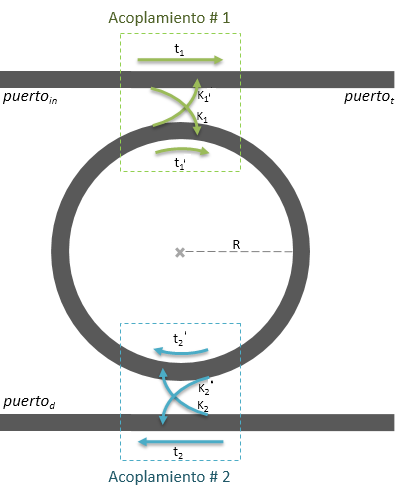
\includegraphics[width=5cm,natwidth=396,natheight=495]{figs/rr_model.PNG}
\label{fig:rr_model}
\end{figure} 

Para que el dispositivo entre en resonancia, el desfase de la onda después de un viaje
completo al rededor del anillo debe ser un múltiplo entero de $2 \pi$

\begin{equation}
\beta L = 2 \pi M
\label{eq:resonant_condition}
\end{equation} 
 
Donde $M$ es llamado el número de modo. 

La potencia de la onda que se ve en el $puerto_t$ está dada por la porción de la onda incidente
que atravieza la guía más las $N\to\infty$ contribuciones que se dan por la otra parte de la
onda que se acopló en el anillo (ec. \ref{eq:coupling_sum}). 
Cada una de las contribuciones depende del número de viajes completos que realice la onda
acoplada antes de volver a salir a la guía superior.

\begin{align}
E_t = E_i\{
t_1+
\kappa_1\kappa_1^{'} t_2^{'} \alpha e^{-j \beta L} [ 
1 +
&(t_1^{'} t_2^{'} \alpha e^{-j \beta L})^1 + \nonumber \\
&(t_1^{'} t_2^{'} \alpha e^{-j \beta L})^2 +
...]\}
\label{eq:coupling_sum}
\end{align}

Resolviendo la serie infinita, normalizando la potencia de salida
 y multiplicando por la correspondiente conjugada 
compleja (recordar que $|\chi|^2 = \chi \chi^*$  \cite{paloczi2005polymer}) se puede llegar a:

\begin{align}
 T_t &= |\frac{E_t}{E_i}|^2 = 
    \frac{\alpha^2 |t_2|^2 + |t_1|^2 - 2\alpha |t_1||t_2| 
	\cos(\theta + \phi_{t_1} + \phi_{t_2}) }
    {1 + \alpha^2|t_1|^2 |t_2|^2 - 2\alpha |t_1||t_2|
	\cos(\theta + \phi_{t_1} + \phi_{t_2}) }
\label{eq:T_t}
\end{align} 


\begin{align}
 T_d &= 
    \frac{\alpha^2 (1-|t_1|)^2 (1-|t_2|)^2}
    {1 + \alpha^2|t_1|^2 |t_2|^2 - 2\alpha |t_1||t_2|
	\cos(\theta + \phi_{t_1} + \phi_{t_2}) }
\label{eq:T_d}
\end{align} 

Donde $\theta = \beta L$. 

Se observa que ocurre una situación especial cuando la suma de los desfases que
sufre la onda en su viaje completo al rededor del anillo es un múltiplo entero
de $2\pi$ (\ref{eq:resonance_condition}). 
Esta condición es llamada condición de resonancia.

\begin{equation}
\theta + \phi_t = 2\pi * M
\label{eq:resonance_condition}
\end{equation} 

Bajo esta condición, la ecuación de transmisión en el $puerto_t$ queda:
\begin{equation}
T_t=\frac{(\alpha - |t|)^2}{(1-\alpha|t|)^2}
\label{eq:t_resonance}
\end{equation} 

A partir de (\ref{eq:t_resonance}) se ve que cuando $\alpha=|t|=\sqrt{1-|\kappa|^2}$ la transmitancia
en el $puerto_t$ es cero. Es decir que cuando las pérdidas en la región de 
acoplamiento son iguales a las pérdidas en el anillo, se llega a la condición
llamada Acoplo Crítico, donde la potencia de salida se anula.

Visto desde el punto de vista de \cite{blasco2011desarrollo} el fenómeno se 
produce porque la longitud de onda que cumple la condición se acopla, sufre un 
desfase de $\frac{\pi}{2}$, es decir $\kappa = i|\kappa|$. 
Luego de completar una vuelta completa sufre un desfase de $2\pi$ y cuando
se vuelve a acoplar a la guía recta es desfasada nuevamente $\frac{\pi}{2}$.
Es decir, que cuando vuelve a la guía inicial, se suma en contrafase en el 
punto de acoplamiento de la guía, anulándola.

\subsection{Simulaciones}
Para la realización de esta etapa de la investigación, se planteó realizar la simulación
de la onda electromagética cuando interactúa con una estructura en anillo con el fin de 
conocer los parámetros que afectan directamente su comportamiento.

Para el caso de prueba el diseño propuesto se eligió el filtro Notch.
Este componente es de extrema importancia ya que es uno de los ladrillos de construcción
de estructuras más complejas que se emplean como filtros, switches banda ancha y detectores.

Las simulaciones se realizaron mediante la técnica de FDTD en 2 plataformas diferentes. 
La primera es una herramienta de software libre llamda MEEP en la cual se codifca un 
script que contiene la información de la estructura a simular.
La segunda es una herramienta comercial llamada Lumerical-FDTD, que cuenta con una interfaz
gráfica de usuario que sirve para controlar el diseño y la ejecución de la simulación, pero
a su vez también cuenta con soporte para scripts con una sintaxis similar a la de matlab 
.

Para el diseño del anillo, se siguieron los lineamientos descritos en \cite{Lumerical2009}
aplicadas sobre el filtro Notch, el cual consiste en
el modelo explicado en la sección anterior con la salvedad que 
la región de Acoplamiento 1 es idéntica a la región de Acoplamiento 2, por lo tanto
$\kappa = \kappa_1 = \kappa_2$, 
$\kappa^* = \kappa_1^* = \kappa_2^*$, 
$t=t_1 = t_2$ y 
$t^*=t_1^* = t_2^*$. 
Adicionalmente, se asume que no hay pérdidas $(\alpha=1)$ y
se seleccionan las características dadas en la tabla \ref{tb:lum_params}.

\begin{table}[H]
\centering
\begin{tabular}{|l|l|}
\hline
Parámetro & Valor \\
\hline
Rango de frecuencias & 1500nm a 1600nm \\ 
$\lambda_0$ & 1550nm \\
Espaciamiento de canales & 200Ghz ó 1.6nm a 1550nm \\
$FSR$ & 3200GHz ó 25.6nm a 1550nm ó 16 canales \\
$\Delta \lambda_{FWHM}$ & 100GHz ó 0.8nm \\
$Q$ & $\frac{1550nm}{0.8nm} \approx 2000$ \\
\hline
\end{tabular}
\caption{Configuración deseada para el filtro}
\label{tb:lum_params}
\end{table} 


Una vez ejecutadas las simulaciones, se obtuvieron las gráficas \ref{fig:meep_res_n} y 
\ref{fig:meep_res_n} en el software de Meep en 2 y 3 dimensiones respectivamente. 
La figura \ref{fig:lum_t_fdtd_n} muestra el resultado de la misma estructura 3D sobre el 
software de Lumerical-FDTD de potencia vs longitud de onda.

La gráfica \ref{fig:meep_res_n} muestra 
\begin{figure}
\caption{Transmitancia Filtro Notch 2D en MEEP. Fuente: Autor.}
\centering
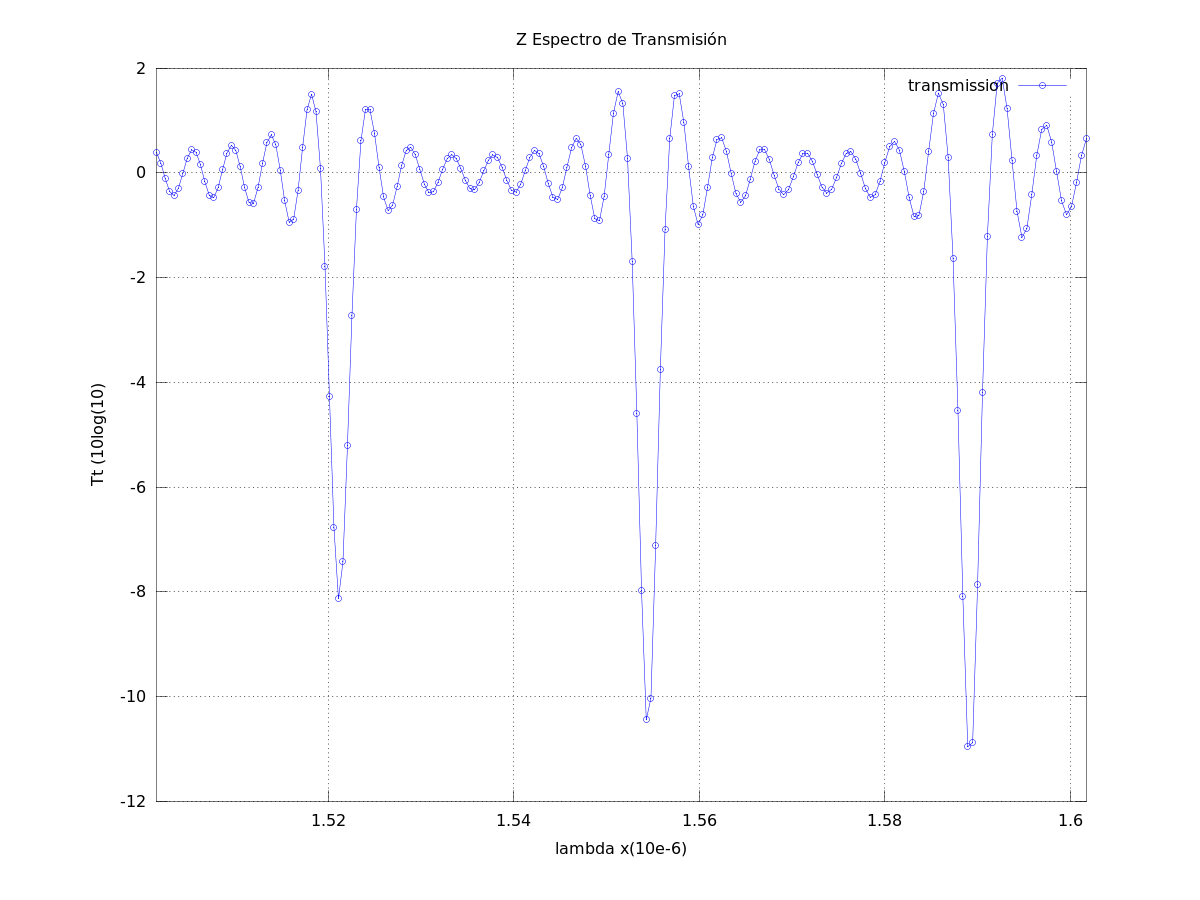
\includegraphics[width=5cm,natwidth=1200,natheight=900]{figs/gausrc_flux_mod-graph_res80.png}
\label{fig:meep_res_n}
\end{figure}

En la figura \ref{fig:notch_geometry} se muestran diferentes vistas de la 
estructura 3D obtenida en MEEP.

\begin{figure}
\caption{Filtro Notch 3d en MEEP: vista [X,Y], [Y,Z] y [X,Z] respectivamente. (a)(b)(c) Material Dieléctrico. (d)(e)(g) Campo eléctrico $E_z$. Fuente: Autor.}
\centering
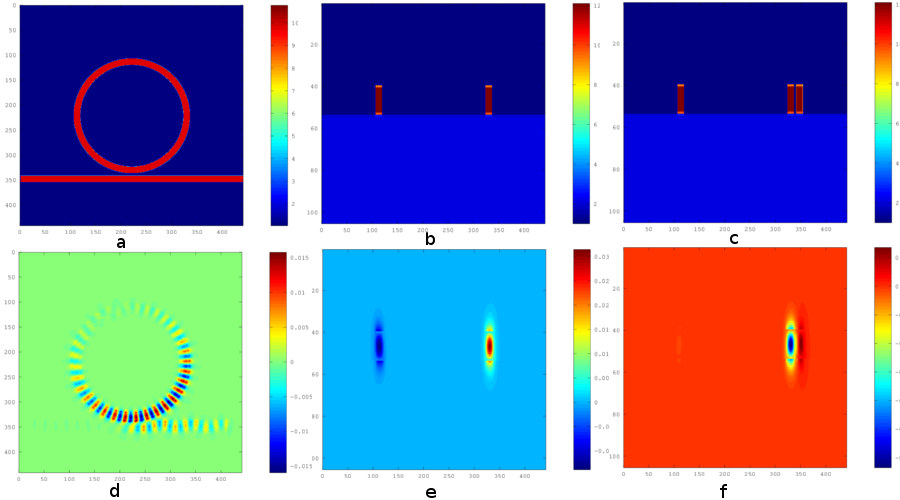
\includegraphics[width=5cm,natwidth=900,natheight=500]{figs/notch3d.png}
\label{fig:notch_geometry}
\end{figure}

\begin{figure}
\caption{Transmitancia Filtro Notch 3D en MEEP. Fuente: Autor.}
\centering
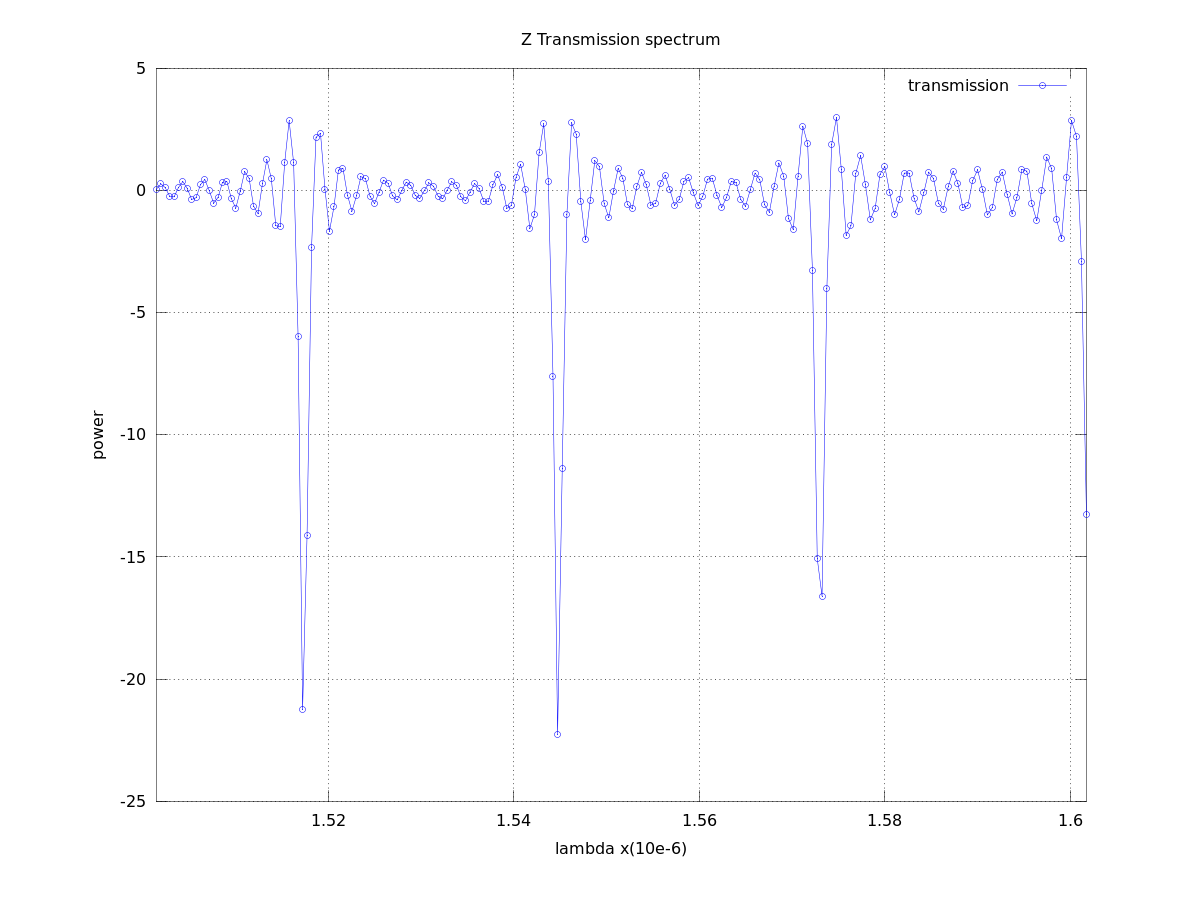
\includegraphics[width=5cm,natwidth=1200,natheight=900]{figs/notch3d_T.png}
\label{fig:meep_res_n}
\end{figure}

\begin{figure}
\caption{Transmitancia simulación 3D FDTD Filtro Notch en LumericalFDTD (valores teóricos, simulación MODE y 
FDTD). Fuente: Autor.}
\centering
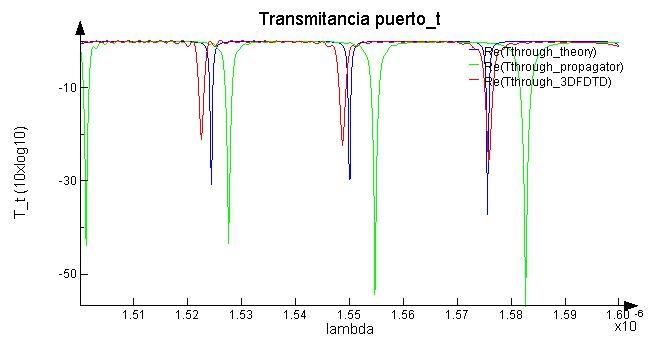
\includegraphics[width=7cm,natwidth=632,natheight=356]{figs/lum_Tt.jpg}
\label{fig:lum_t_fdtd_n}
\end{figure} 

Se pueden observar diferencias en cuanto al valor teórico esperado en las
condiciones de resonancia para todas las simulaciones,
debido a que se asumió que el anillo no presentaba pérdidas $(\alpha = 1)$ en
el cálculo teórico de la transmitancia.

Sin embargo, la que más difiere de todas inclusive en el FSR esperado 
es la simulación mostrada en la figura \ref{fig:meep_res_n}. Esto se puede deber a
que esta simulación se realizó sólamente en 2 dimensiones y por lo tanto
deja de lado la interacción de la onda con el materia de Sílica SiO2.

\section{Redes de Interconexión}
En esta fase de la investigación, se planteó realizar la simulación de 
una red de interconexión electrónica y nanofotónica híbrida para 
realizar la comparación del desempeño en términos de latencia y consumo
de energía en 5x2 diferentes escenarios.

Para cada escenario se obtuvo el tamaño de la muestra requerido
para obtener un nivel de confianza del 95\%. Luego se procedió
a definir la comparación para cada variable a medir, 
mediante la prueba de hipótesis para comparación de medias. 

La red consta de 2 planos independientes: procesamiento y
red de interconexión fotónica híbrida conmutada. 

El plano de procesamiento está compuesto por 64 
cores en un arreglo de 8x8. 

Como se indica en \cite{dally2004principles}, una red de interconexión está definida
por 3 características principales: la topología empleada, el algoritmo de control de
flujo y el algoritmo de ruteo. La red de interconexión simulada en este experimento
consta de una topología Mesh con concentración de nodos ó C-Mesh (Figura \ref{fig:cmesh}), 
de un algoritmo de control de
flujo llamado \textit{Bubble Flow Control}\cite{puente1999adaptive}\cite{Manual} y
de un algoritmo de enrutamiento basado en un esquema direccionamiento jerárquico
basado en direcciones de la forma $NET.PROC$ como se explica en \cite{Manual}.

\begin{figure}
\caption{Topología C-Mesh. Fuente: \cite{Manual}}
\centering
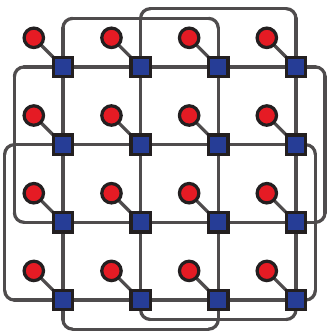
\includegraphics[width=4cm,natwidth=333,natheight=336]{figs/cmesh.png}
\label{fig:cmesh}
\end{figure} 

Debido a la topología concentrada que se seleccionó, la red de interconexión 
está compuesta por 4x4 elementos, donde cada nodo terminal da servicio al 
número dado por el parámetro de concentración, que para esta simulación se estableció
en 4.

Sobre cada red se ejecutaron las siguentes aplicaciones sintéticas 
(Figura \ref{fig:synthbench}):
\begin{itemize}
\item Random: 
Ejecuta un tráfico aleatorio sobre la red. Cada core selecciona un core destino aleatoriamente
mediante una distribución uniforme. Una vez enviado, espera un tiempo dado por el parámetro
\textit{appParam1} para enviar un nuevo mensaje \cite{Manual}.

\item Neighboor: 
Realiza el envío de mensajes de cada core a sus vecinos \cite{hendry2009analysis}.

\item BitReverse: 
Patrón de envío de mensajes diseñado para realizar pruebas de estrés sobre topologías NoC 2D.
Cada core envía un mensaje a una dirección que corresponde a su dirección inversa a nivel de
bits. Este tipo de comunicación, los mensajes deben viajar trayectos largos que atraviezan la 
red \cite{hendry2009analysis}.

\item Tornado: 
Otro patrón de envío de mensajes que realiza pruebas de estrés sobre Mesh 2D al hacer que
cada core se comunique con el vecino de su vecino. Es una versión competitiva del patrón
Neighboor \cite{hendry2009analysis}.
\end{itemize}
 
\begin{figure}[H]
\caption{Patrones sintéticos. Fuente \cite{hendry2009analysis}}
\centering
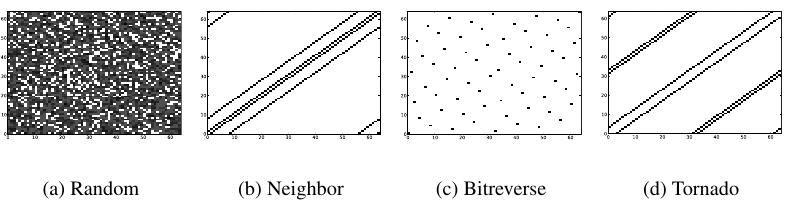
\includegraphics[width=6cm,natwidth=787,natheight=205]{figs/syntbench.png}
\label{fig:synthbench}
\end{figure} 


El promedio de tiempo de generación de mensajes se escogió de 1 milisegundo. 
Adicionalmente,
para cada red y para cada aplicación, se decidió realizar la simulación
con 2 tamaños de mensajes (pequeño: 512Bytes y grande:65kBites) entre núcleos,
siguiendo la metodología empleada en \cite{hendry2009analysis}.
\subsection{Paquetes Pequeños (512B)}

En las tablas \ref{tb:eall512} y \ref{tb:lall512} se sintetizan 
las medias del consumo de energía y de
latencia para los mensajes pequeños.

\begin{table}[]
\centering
\begin{tabular}{|c|c|c|c|}
\hline
&Electrónica&íbrida Fotónica\\
\hline
Neighboor&0.06709065&0.007958905\\
Random&0.0671371&0.007956592\\
BitReverse&0.067138183&0.00795793\\
otSpot&0.067167386&0.007965599\\
Tornado&0.067086057&0.007954494\\
\hline
\end{tabular}
\caption{Datos promedio Consumo de Energía $(J)$, PkgSize: 512B}
\label{tb:eall512}
\end{table}


\begin{table}[]
\centering
\begin{tabular}{|c|c|c|c|}
\hline
&Electrónica&íbrida Fotónica\\
\hline
Neighboor&0.069082133&0.079211817\\
Random&0.08788594&0.1318324\\
BitReverse&0.116597833&0.201336333\\
otSpot&0.092226286&0.139719571\\
Tornado&0.070975529&0.086788314\\
\hline
\end{tabular}
\caption{Datos promedio Latencia $(\mu s)$, PkgSize: 512B}
\label{tb:lall512}
\end{table}

Se puede observar gráficamente que el consumo de energía de la red
nanofotónica híbrida es mucho menor que el de la red netamente electrónica.
Sin embargo, la variable de latencia muestra que para este tipo de mensajes
la red fotónica híbrida se comporta peor que la red electrónica.

\begin{figure}[]
\caption{Comparación Consumo de Energía, PkgSize: 512B. Fuente: Autor.}
\centering
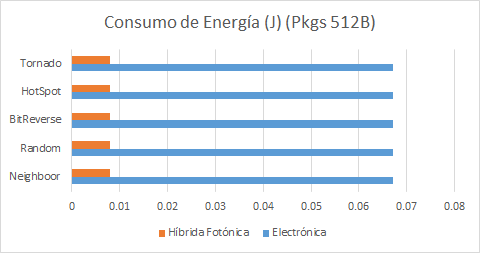
\includegraphics[width=8cm,natwidth=483,natheight=256]{figs/E512.png}
\label{fig:e512}
\end{figure} 

\begin{figure}[]
\caption{Comparación Latencia, PkgSize: 512B. Fuente: Autor.}
\centering
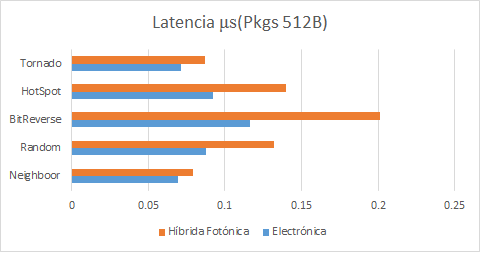
\includegraphics[width=8cm,natwidth=483,natheight=256]{figs/L512.png}
\label{fig:l512}
\end{figure} 

Los resultados de las pruebas de hipótesis se presentan a continuación:
 
\begin{table}[]
\centering
\begin{tabular}{|c|c|c|c|}
\hline
&Valor P&Rechaza $H_0$ ?\\
\hline
Neighboor&7.29052E-32&TRUE\\
Random&2.21789E-23&TRUE\\
BitReverse&2.85143E-29&TRUE\\
otSpot&1.42176E-32&TRUE\\
Tornado&3.3077E-41&TRUE\\
\hline
\end{tabular}
\caption{Resultados Prueba Hipótesis para la variable Consumo de Energía, PkgSize: 512B}
\label{tb:ettest512}
\end{table}

En la tabla \ref{tb:ettest512} se encontró que en todos los casos se presentó una
respuesta positiva. Esto se puede concluir debido a que el valor P para
en todos los resultados fue mayor a 0.05 y por lo tanto se puede concluir que 
la red nanofotónica híbrida sí es mejor en términos de consumo de potencia
que la red electrónica analizada para tamaños de mensajes pequeños.


\begin{table}[]
\centering
\begin{tabular}{|c|c|c|c|}
\hline
&Valor P&Rechaza $H_0$ ?\\
\hline
Neighboor&0.99999883&FALSE\\
Random&1&FALSE\\
BitReverse&1&FALSE\\
otSpot&0.999989&FALSE\\
Tornado&0.9999999&FALSE\\
\hline
\end{tabular}
\caption{Resultados Prueba Hipótesis para la variable Latencia, PkgSize: 512B}
\label{tb:lttest512}
\end{table}

En la tabla \ref{tb:lttest512} se puede confirmar lo observado
gráficamente para la variable de 
latencia. En los paquetes de mensajes pequeños,
no hay evidencias suficientes para afirmar que la red fotónica
es mejor que la electrónica. Es más, en todos los casos se comportó peor.

Este resultado se puede entender desde el punto de vista de la red híbrida,
ya que al necesitar un subplano de control electrónico para hacer el \textit{setup} del
camino antes de enviar los datos por el subplano fotónico. Cuando los mensajes son
pequeños, el sobrecosto de realizar este trabajo sobrepasa en gran medida el 
beneficio de tener una red de transmisión fotónica \cite{shacham2008photonic} y por lo tanto no
logra el rendimiento esperado.

\subsection{Tamaño de Paquetes Grande (65kB)}

En las tablas \ref{tb:eall65k} y \ref{tb:lall65k} se sintetizan 
las medias del consumo de energía y de
latencia para los mensajes grandes (65kB).

\begin{table}[]
\centering
\begin{tabular}{|c|c|c|c|}
\hline
&Electrónica&Híbrida Fotónica\\
\hline
Neighboor&0.0671522&0.007992393\\
Random&0.067220125&0.007997565\\
BitReverse&0.067238325&0.008002103\\
otSpot&0.067256343&0.008007099\\
Tornado&0.067128414&0.007989729\\
\hline
\end{tabular}
\caption{Datos promedio Consumo de Energía $(J)$, PkgSize: 65kB}
\label{tb:eall65k}
\end{table}


\begin{table}[]
\centering
\begin{tabular}{|c|c|c|c|}
\hline
&Electrónica&Híbrida Fotónica\\
\hline
Neighboor&1.399546667&0.322496\\
Random&1.5103925&0.52517175\\
BitReverse&1.5527575&0.610555\\
otSpot&1.582484286&0.536560857\\
Tornado&1.436545714&0.388274\\
\hline
\end{tabular}
\caption{Datos promedio Latencia $(\mu s)$, PkgSize: 65kB}
\label{tb:lall65k}
\end{table}

Nuevamente se puede observar gráficamente que el consumo de energía de la red
nanofotónica híbrida es mucho menor que el de la red netamente electrónica.
Sin embargo, en este caso, la variable de latencia SI muestra que 
para este tipo de mensajes la red fotónica híbrida se comporta mucho mejor 
que la red electrónica.

\begin{figure}[]
\caption{Comparación Consumo de Energía, PkgSize: 65kB. Fuente: Autor.}
\centering
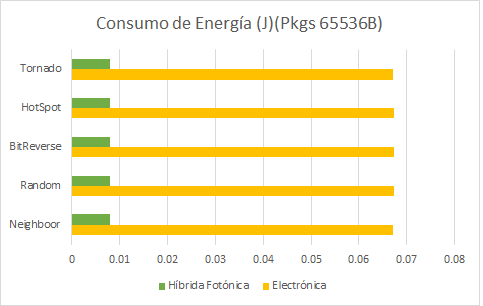
\includegraphics[width=8cm,natwidth=483,natheight=306]{figs/E65k.png}
\label{fig:e65k}
\end{figure} 

\begin{figure}[]
\caption{Comparación Latencia, PkgSize: 65kB. Fuente: Autor.}
\centering
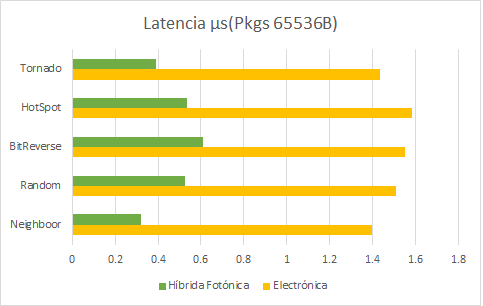
\includegraphics[width=8cm,natwidth=483,natheight=306]{figs/L65k.png}
\label{fig:l65k}
\end{figure} 

\begin{table}[]
\centering
\begin{tabular}{|c|c|c|c|}
\hline
&Valor P&Rechaza $H_0$ ?\\
\hline
Neighboor&2.427440e-22 TRUE&TRUE\\
Random&1.05729E-17&TRUE\\
BitReverse&2.41872E-20&TRUE\\
otSpot&1.57746E-32&TRUE\\
Tornado&5.3047E-39&TRUE\\
\hline
\end{tabular}
\caption{Resultados Prueba Hipótesis para la variable Consumo de Energía, PkgSize: 65kB}
\label{tb:ettest65k}
\end{table}

En la tabla \ref{tb:ettest65k} se puede observar en todos los casos una
respuesta positiva debido a que el valor P para
todos los resultados fue mayor a 0.05. Por lo tanto, también se puede concluir que 
la red nanofotónica híbrida sí es mejor en términos de consumo de potencia
que la red electrónica analizada para tamaños de mensajes grandes.

\begin{table}[]
\centering
\begin{tabular}{|c|c|c|c|}
\hline
&Valor P&Rechaza $H_0$ ?\\
\hline
Neighboor&7.08709E-14&TRUE\\
Random&5.37024E-10&TRUE\\
BitReverse&3.01947E-11&TRUE\\
otSpot&2.99509E-16&TRUE\\
Tornado&8.35414E-21&TRUE\\
\hline
\end{tabular}
\caption{Resultados Prueba Hipótesis para la variable Latencia, PkgSize: 65kB}
\label{tb:lttest65k}
\end{table}

En la tabla \ref{tb:lttest65k} también se encontró en todos los casos una
respuesta positiva. Es decir que para tamaños de mensajes grandes, el sobrecosto
de la subred de control es insignificante en cuanto a las mejoras obtenidas
en latencia por el subplano fotónico de transmisión de datos.


\section{Conclusiones}
\begin{itemize}
\item Las frecuencias de resonancia del anillo pueden ser manipuladas mediante
modificaciones en el diámetro del anillo, el gap o el índice de refracción. Este
último es de gran importancia por ser la base del funcionamiento algunos dispositivos
moduladores en Silicon Photonics donde se aplica un campo
magnético, generando un efecto plasmónico que altera el índice y por lo tanto
los modos de resonancia.
\item Debido a que se asumió que el anillo no presentaba pérdidas $(\alpha = 1)$ en
el cálculo teórico de la transmitancia tanto del filtro Notch como del filtro
AddDrop, se pueden apreciar diferencias en las condiciones de resonancia
de la teoría con respecto a lo obtenido en la práctica.
\item Para tamaños de mensajes grandes, la red de interconexión nanofotónica
híbrida C-Mesh se comporta mejor en términos de consumo de energía y latencia
que la red electrónica C-Mesh.
\item  Para tamaños de mensajes grandes, la red de interconexión nanofotónica
híbrida C-Mesh se comporta mejor únicamente en términos de consumo de energía 
que la red electrónica C-Mesh.
\item  En los paquetes de mensajes pequeños,
no hay evidencias suficientes para afirmar que la red fotónica
es mejor que la electrónica en la variable de latencia debido a que
el sobrecosto de la subred de control electrónica realizar 
sobrepasa en gran medida el beneficio de tener una red de transmisión fotónica 
y por lo tanto no logra el rendimiento esperado.
\end{itemize} 

\section{Trabajos Futuros}
\begin{itemize}
\item Como trabajo futuro se plantea realizar nuevas simulaciones para los dos
filtros modificando el diámetro del anillo para visualizar 
la alteración en el FSR y su uso como filtro selectivo o filtro de banda ancha.
\item Se propone también, para un diámetro fijo, realizar simulaciones alterando 
el índice de refracción del anillo para simular el efecto plasmónico que 
sucede dentro del modulador y que hace que se desplacen las frecuencias de resonancia
de un estado On a Off.
\item Se plantea como trabajos futuros, evaluar otras topologías en
la red de interconexión, así como ampliar la prueba ejecutando también
el subgrupo de aplicaciones científicas.
\item Debido a los resultados obtenidos para mensajes pequeños en términos de 
latencia, sería ideal probar otros tipos de redes implementadas
diferentes a las híbridas conmutadas, es decir, que no tengan un subplano
de control electrónico. Por ejemplo la TDM arbitrada por longitud de onda
descrito en \cite{hendry2011time} o \cite{vantrease2008corona}.
\item Fortalecer los benchmark con los que se analiza el rendimiento de las redes
electrónicas y nanofotónicas en PhoenixSim, abarcando un espectro más amplio
de aplicaciones que involucren áreas como Machine Learning, Software de Base de Datos,
Computación Gráfica y Juegos.
\end{itemize} 

\section{Agradecimientos}
Agradecimientos a Colciencias por su apoyo a este proyecto
a través del programa Jóvenes Investigadores e Innovadores 2011
del cual fue beneficiaria la investigadora Tatiana López.

Igualmente la colaboración de los integrantes del grupo Sirius, tanto
técnica como personal, fue indispensable para lograr los objetivos 
propuestos.

\bibliographystyle{plain}
\bibliography{biblio}

\end{document}
